\section{Task Clarification}
Until now a model was developed and with this model settings for a PID controller were found. To test these settings on the real BalanBot, a Simulink model which implements the hardware specific functions is needed. This includes reading the acceleration and gyroscope sensors, filtering and processing them and writing to the output registers. This ensures that the BalanBot also moves in a different direction with a negative output of the controller than with a positive output. 

\section{Detailed Code Commentary}
\subsection{Sensor Data Reading}
The IMU communicates with the Arduino via the I2C bus. This must be implemented in the Simulink design. The sensor values obtained from this must now be further ground via Matlab function blocks. To get more trustworthy data in the later course of the program, a Kalman filter was also used. However, this filter needs both the measured angle and the measured yaw rate for proper operation. Therefore these two values were calculated. 

\begin{figure}[H]
    \centering
    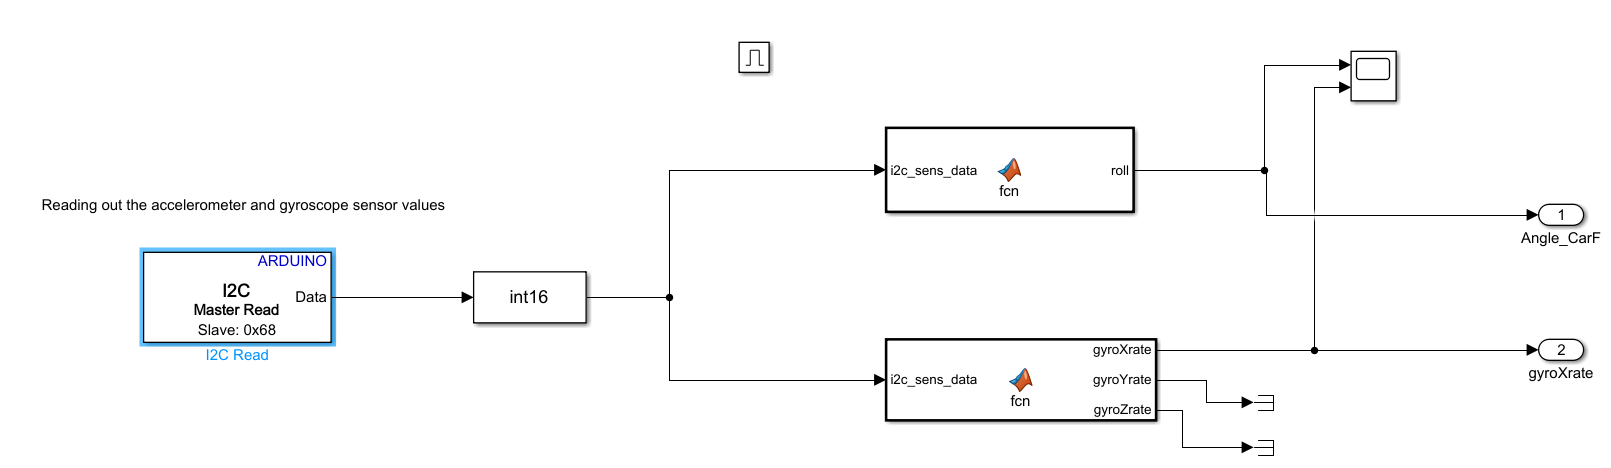
\includegraphics[width=\textwidth]{Lab_report/pics/hardware_impl/gyro_read.PNG}
    \caption{data reading Submodel}
    \label{fig:acc_gyro_read}
\end{figure}

\begin{lstlisting}[language=Matlab, caption=angle calculation]
function roll = fcn(i2c_sens_data)
    accX = double(i2c_sens_data(1));
    accY = double(i2c_sens_data(2));
    accZ = double(i2c_sens_data(3));
    roll = atan(accY / sqrt(accX * accX + accZ * accZ)) * 180/pi; 
end
\end{lstlisting}

\begin{lstlisting}[language=Matlab, caption=gyro rate calculation]
function [gyroXrate,gyroYrate,gyroZrate] = fcn(i2c_sens_data)
    gyroX = double(i2c_sens_data(5));
    gyroY = double(i2c_sens_data(6));
    gyroZ = double(i2c_sens_data(7));
    gyroXrate = gyroX/131;
    gyroYrate = gyroY/131;
    gyroZrate = gyroZ/131; 
end
\end{lstlisting}

\subsection{Data Processing}
In this submodel, the determined data is first filtered by a Kalman filter and then fed to the control algorithm. The data processing by means of this filter is described in more detail below.
\subsubsection{Kalman filter}
The principle of this filter is based on the estimation of the output quantity and the comparison of the measured output quantity. The difference of these two quantities is then weighted with the Kalman gain and used to correct the estimated output value. In our case the code for this estimation and correction algorithm is already finished and only a small test and proof of concept will be shown here. 

\subsubsection{Controller}
To control the BalanBot, a PID controller was implemented after the Kalman filter.
\begin{figure}[H]
    \centering
    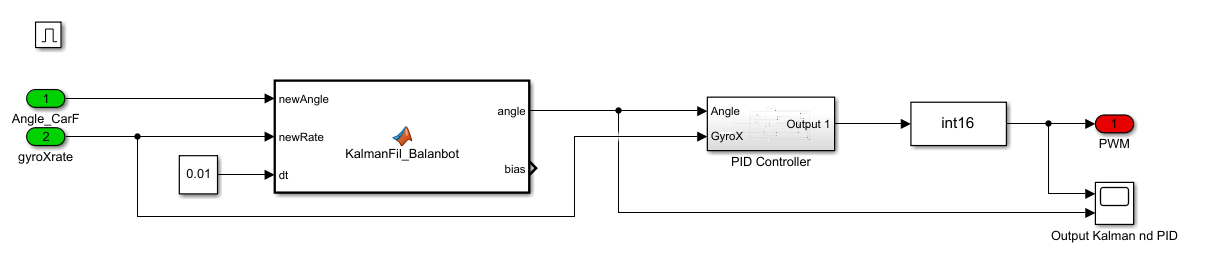
\includegraphics[width=\textwidth]{Lab_report/pics/hardware_impl/motor-control.PNG}
    \caption{Model of the Motor Control}
    \label{fig:motor control model}
\end{figure}

The PID-Controller Submodel looks as can be seen in \autoref{fig:pid_model}.
\begin{figure}[H]
    \centering
    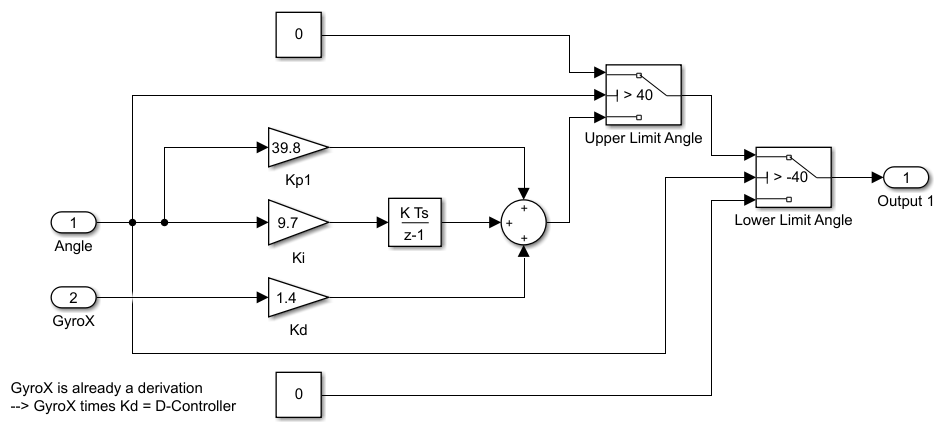
\includegraphics[width=\textwidth]{Lab_report/pics/hardware_impl/PID.PNG}
    \caption{Model of the PID Controller}
    \label{fig:pid_model}
\end{figure}
To 
The angle limit was also implemented into the PID-Controller Submodel. If the angle of the BalanBot is bigger than $40^\circ$ or smaller than $-40^\circ$ , the output (= motor speed) gets set to 0RPM.
\newline\\\\
\textbf{Adjusting of the PID-Controller gains}\\\\
The settings of the PID controller had already been estimated by using the Simulink model beforehand. However, when testing these settings on the real BalanBot, the PID-Controller could not stabilize the BalanBot.\\\\
To obtain some reasonable PID-Controller parameter values, all gains have been initially set to zero. Then, the proportional gain was estimated at first. To get rid of the steady-state-error, a integral gain was also estimated and implemented. However, the BalanBot reacted way too aggressive to faster errors, hence a derivative gain was estimated and implemented.\\\\
The fine tuning of the controller was done in the following order:
\begin{itemize}
    \item Adjusting the proportional gain until the outcome was somewhat nearly satisfactory
    \item Adjusting the integral gain in combination with the proportional gain so the BalanBot would react fast enough but not too strong to errors
    \item Adjusting the derivative gain to smooth the aggressiveness of the controller
\end{itemize}

The final PID-Controller gains can be seen in \autoref{fig:pid_model}.
\subsection{Motor Control}
